\section{Implementierung einer k-Nearest-Neighbors-Suche in Python}


\subsection{
    Implementierung der Python-Funktion \textit{getKNearestNeighbor(X, x, k=1)}
}

\begin{figure}[H]
    \centering
    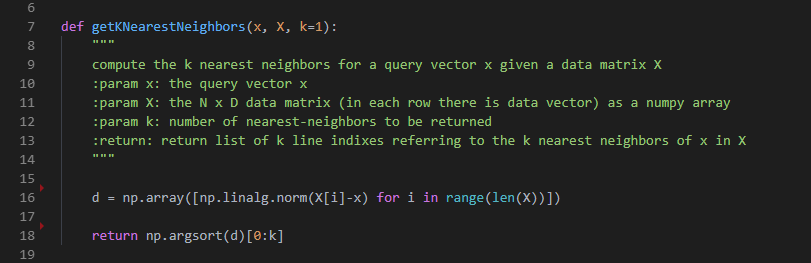
\includegraphics[width=1\linewidth]{files/aufgabe1a.png}
    \caption{Python-Funktion \textit{getKNearestNeighbor()}}
\end{figure}

\subsection{Test der implementierten Python-Funktion}

\begin{figure}[H]
    \centering
    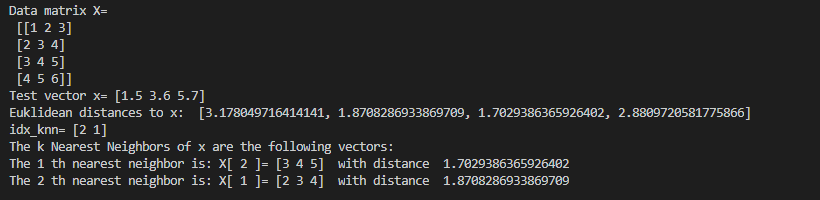
\includegraphics[width=1\linewidth]{files/aufgabe1b.png}
    \caption{Test der Funktion}
\end{figure}

\subsection{Angabe der Rechenschritte in O-Notation}

Es muss für jeden Vektor in X die euklidische Distanz bestimmt werden.
D. h. n Durchläufe.
Weiterhin muss die Funktion \textit{np.argsort()} die zuvor ermittelten
euklidischen Distanzen sortieren, um den Index der kleinsten zurückzuliefern.
Daraus folgt: $O(n + n * log(n))$ unter Annahme, dass \textit{np.argsort()} 
mit Merge-Sort oder Heap-Sort aufgerufen wird, und die Laufzeit somit $n * log(n)$ beträgt.

\noindent
Ein schnelleres Verfahren ginge über den KD-Tree.